\documentclass{article}
\usepackage{tikz}
\usepackage{pgfplots}
\usepackage{textcomp}
\usepackage{array}
\usepackage{tabu}
\usepackage{numprint}
\begin{document}
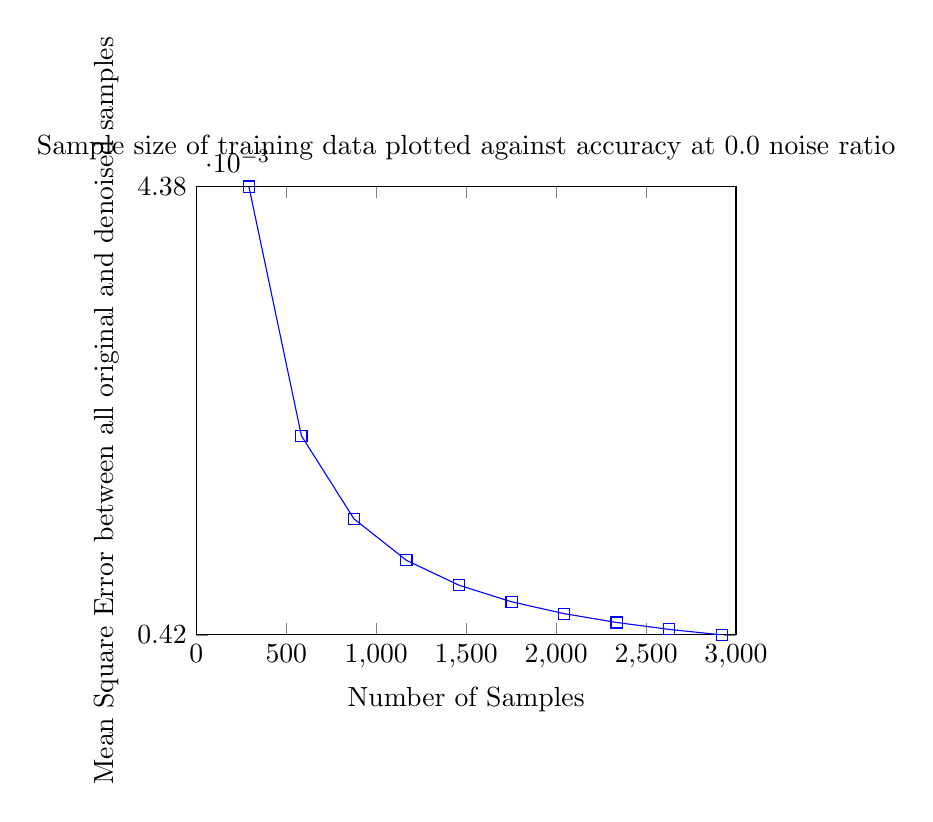
\begin{tikzpicture}
\begin{axis}[
title={Sample size of training data plotted against accuracy at 0.0 noise ratio},
xlabel={Number of Samples},
ylabel={Mean Square Error between all original and denoised samples},
xmin=0, xmax=3000,
ymin=0.0004187208884702004, ymax=0.004384264930605824,
xtick={0,500,1000,1500,2000,2500,3000},
ytick={0.0004187208884702004,0.004384264930605824},
legend pos=north west,
ymajorgrids=true,
grid style=dashed,
]

\addplot[
color=blue,
mark=square,
]
coordinates {

(292, 0.004384264930605824)
(584, 0.002179933016905802)
(876, 0.0014453812510302347)
(1168, 0.0010782827192537564)
(1460, 0.000858155872153815)
(1752, 0.0007115019971104757)
(2044, 0.0006068416122018855)
(2336, 0.0005284441673549079)
(2628, 0.0004675207725913472)
(2921, 0.0004187208884702004)
    };
\end{axis}
\end{tikzpicture}



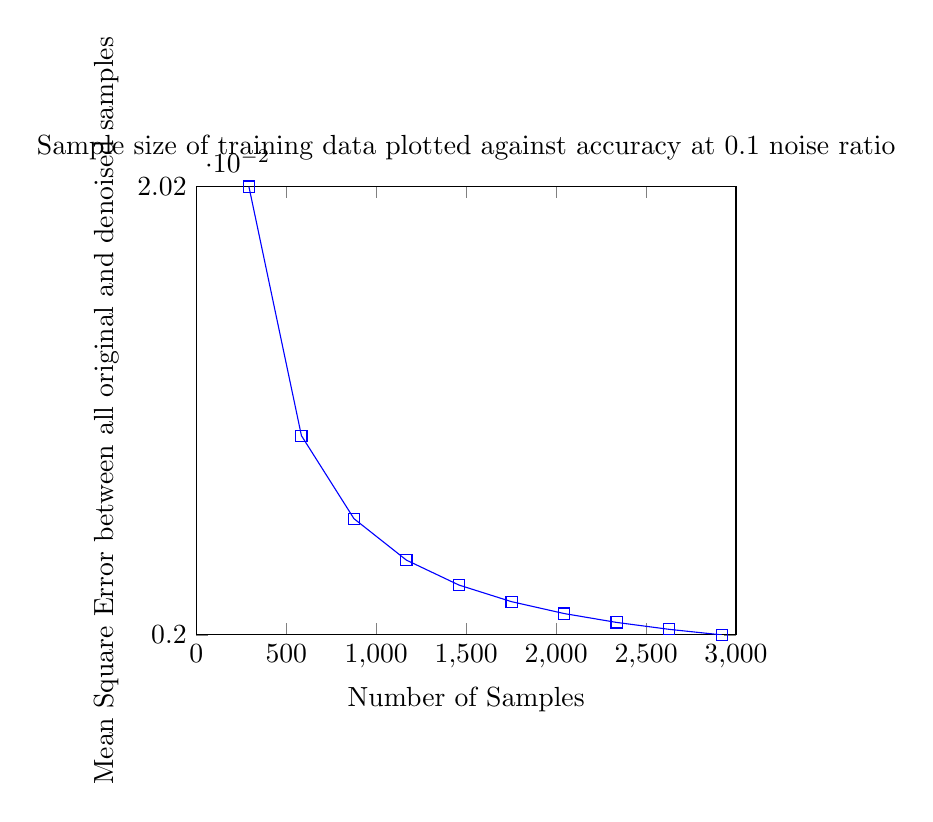
\begin{tikzpicture}
\begin{axis}[
title={Sample size of training data plotted against accuracy at 0.1 noise ratio},
xlabel={Number of Samples},
ylabel={Mean Square Error between all original and denoised samples},
xmin=0, xmax=3000,
ymin=0.0020143148258401967, ymax=0.02018576282803745,
xtick={0,500,1000,1500,2000,2500,3000},
ytick={0.0020143148258401967,0.02018576282803745},
legend pos=north west,
ymajorgrids=true,
grid style=dashed,
]

\addplot[
color=blue,
mark=square,
]
coordinates {

(292, 0.02018576282803745)
(584, 0.01009068281606921)
(876, 0.006725671857652396)
(1168, 0.00504320107884075)
(1460, 0.004033738680451314)
(1752, 0.003360792138314125)
(2044, 0.0028801280452402963)
(2336, 0.002519645208428151)
(2628, 0.002239283320213713)
(2921, 0.0020143148258401967)
    };
\end{axis}
\end{tikzpicture}

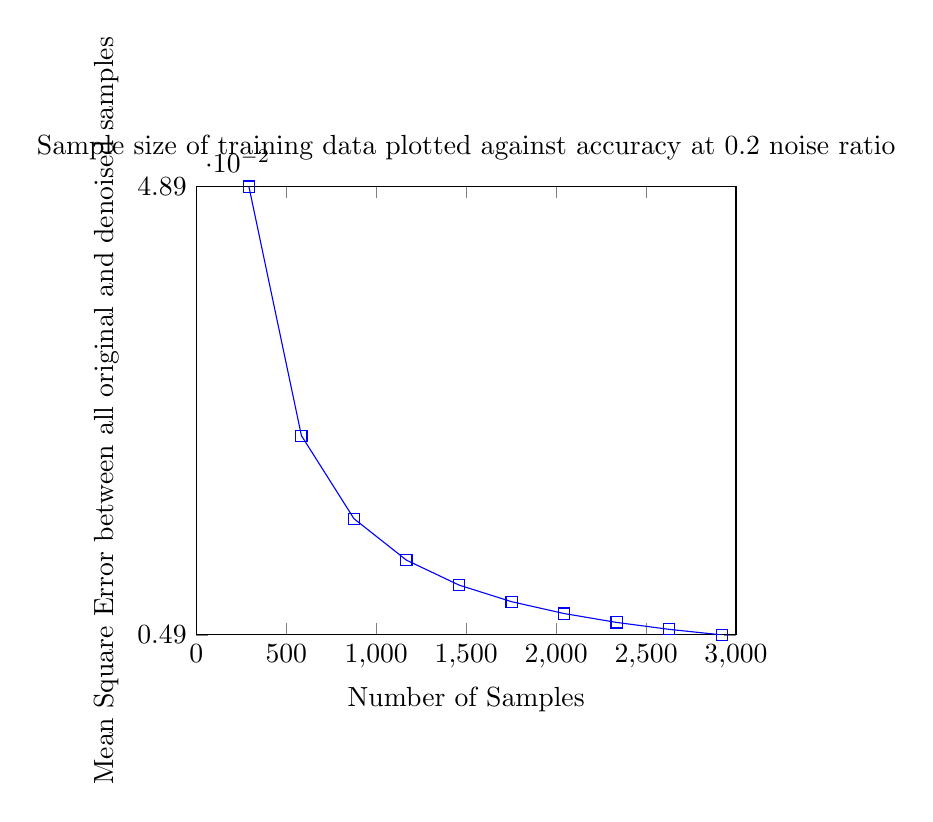
\begin{tikzpicture}
\begin{axis}[
title={Sample size of training data plotted against accuracy at 0.2 noise ratio},
xlabel={Number of Samples},
ylabel={Mean Square Error between all original and denoised samples},
xmin=0, xmax=3000,
ymin=0.0048733088546880415, ymax=0.04888615819375315,
xtick={0,500,1000,1500,2000,2500,3000},
ytick={0.0048733088546880415,0.04888615819375315},
legend pos=north west,
ymajorgrids=true,
grid style=dashed,
]

\addplot[
color=blue,
mark=square,
]
coordinates {

(292, 0.04888615819375315)
(584, 0.024434827253072618)
(876, 0.016284487831684197)
(1168, 0.012209412698153095)
(1460, 0.009764440313161794)
(1752, 0.008134491548192145)
(2044, 0.006970302140571462)
(2336, 0.006097204016321827)
(2628, 0.0054181783028525365)
(2921, 0.0048733088546880415)
    };
\end{axis}
\end{tikzpicture}

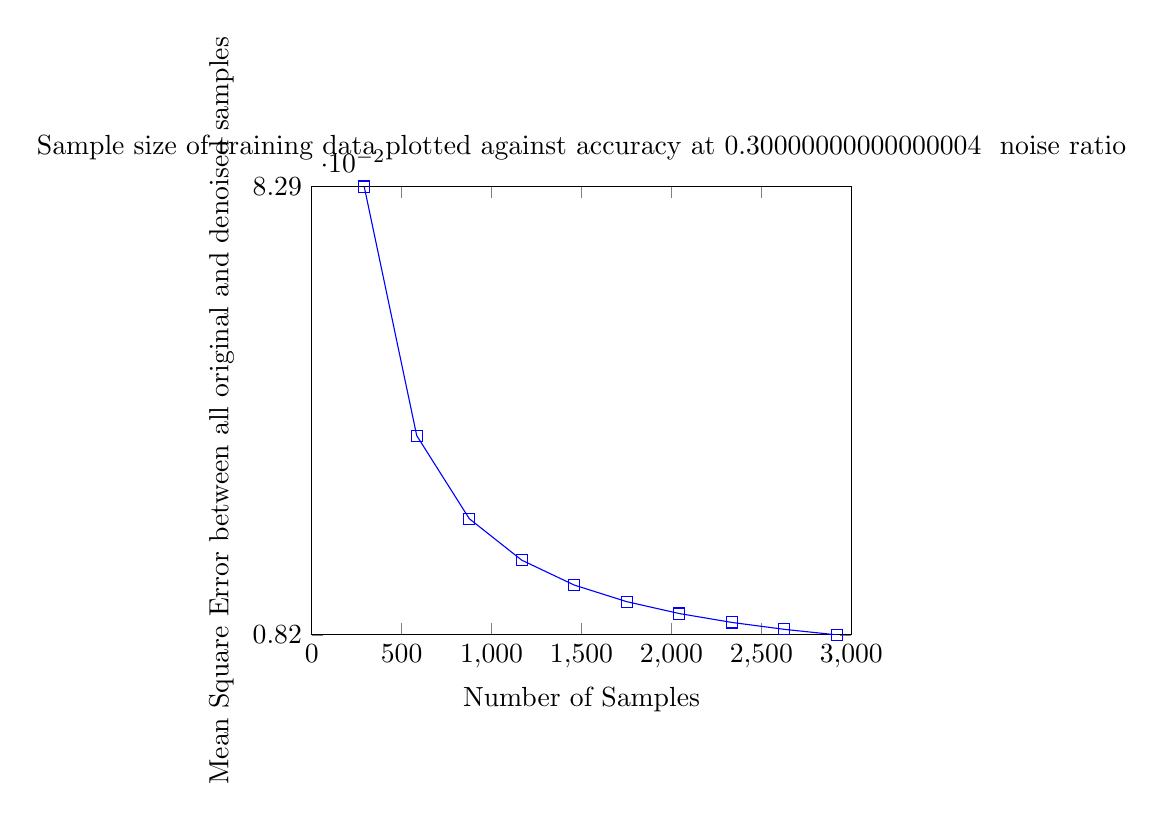
\begin{tikzpicture}
\begin{axis}[
title={Sample size of training data plotted against accuracy at 0.30000000000000004 \
noise ratio},
xlabel={Number of Samples},
ylabel={Mean Square Error between all original and denoised samples},
xmin=0, xmax=3000,
ymin=0.0082226182563895, ymax=0.08291145005879944,
xtick={0,500,1000,1500,2000,2500,3000},
ytick={0.0082226182563895,0.08291145005879944},
legend pos=north west,
ymajorgrids=true,
grid style=dashed,
]

\addplot[
color=blue,
mark=square,
]
coordinates {

(292, 0.08291145005879944)
(584, 0.0414147107722874)
(876, 0.02758308141585993)
(1168, 0.020667742526766224)
(1460, 0.016519054115385286)
(1752, 0.013753676726655487)
(2044, 0.011778766251367444)
(2336, 0.010297874245018756)
(2628, 0.009146376436498845)
(2921, 0.0082226182563895)
    };
\end{axis}
\end{tikzpicture}

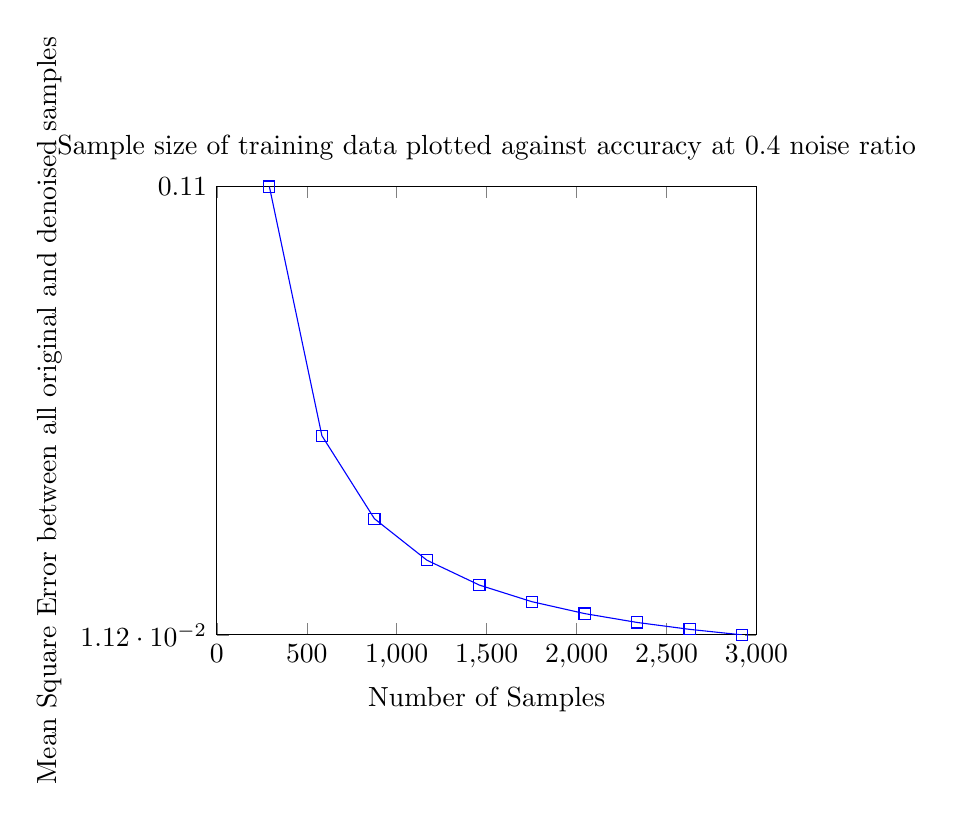
\begin{tikzpicture}
\begin{axis}[
title={Sample size of training data plotted against accuracy at 0.4 noise ratio},
xlabel={Number of Samples},
ylabel={Mean Square Error between all original and denoised samples},
xmin=0, xmax=3000,
ymin=0.011222119821285391, ymax=0.11341628776124728,
xtick={0,500,1000,1500,2000,2500,3000},
ytick={0.011222119821285391,0.11341628776124728},
legend pos=north west,
ymajorgrids=true,
grid style=dashed,
]

\addplot[
color=blue,
mark=square,
]
coordinates {

(292, 0.11341628776124728)
(584, 0.056629424889014984)
(876, 0.037702693521319317)
(1168, 0.028241302162148582)
(1460, 0.022565946683564337)
(1752, 0.01878362640890526)
(2044, 0.01608303102575557)
(2336, 0.014058443884050467)
(2628, 0.012484483426609239)
(2921, 0.011222119821285391)
    };
\end{axis}
\end{tikzpicture}


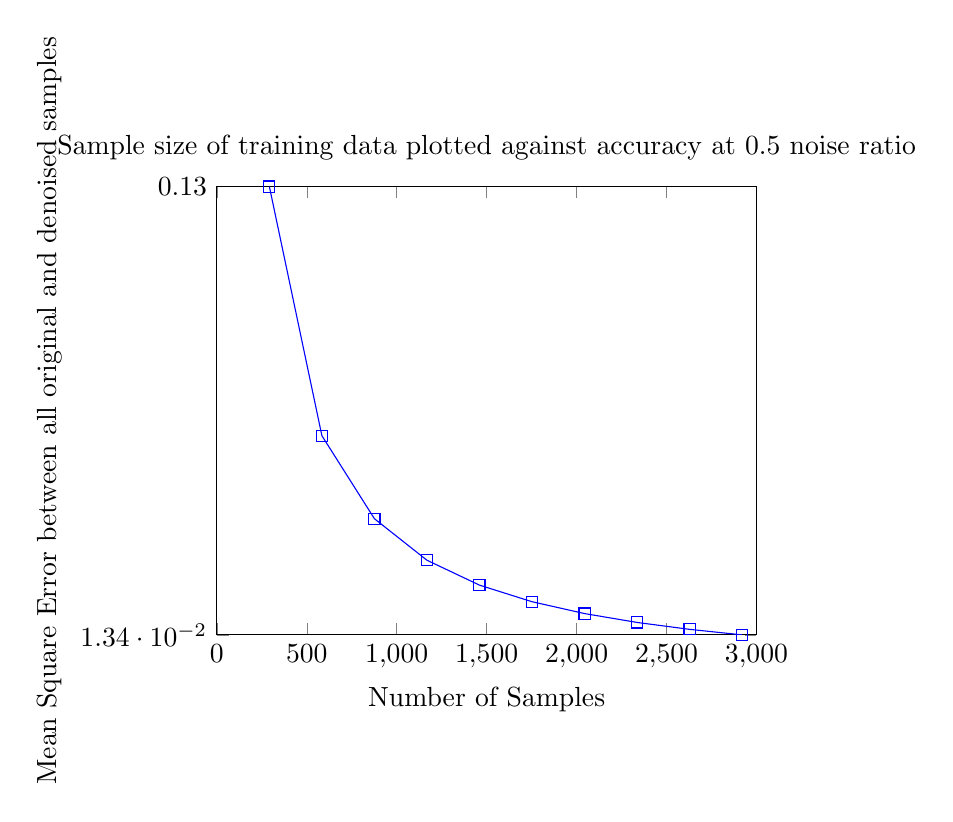
\begin{tikzpicture}
\begin{axis}[
title={Sample size of training data plotted against accuracy at 0.5 noise ratio},
xlabel={Number of Samples},
ylabel={Mean Square Error between all original and denoised samples},
xmin=0, xmax=3000,
ymin=0.013367389392759721, ymax=0.13479311649770576,
xtick={0,500,1000,1500,2000,2500,3000},
ytick={0.013367389392759721,0.13479311649770576},
legend pos=north west,
ymajorgrids=true,
grid style=dashed,
]

\addplot[
color=blue,
mark=square,
]
coordinates {

(292, 0.13479311649770576)
(584, 0.06731768977320013)
(876, 0.04482963665625357)
(1168, 0.03358828472318351)
(1460, 0.026845441555194128)
(1752, 0.022351687145300614)
(2044, 0.019143087780691324)
(2336, 0.0167375686224594)
(2628, 0.014867433494162157)
(2921, 0.013367389392759721)
    };
\end{axis}
\end{tikzpicture}

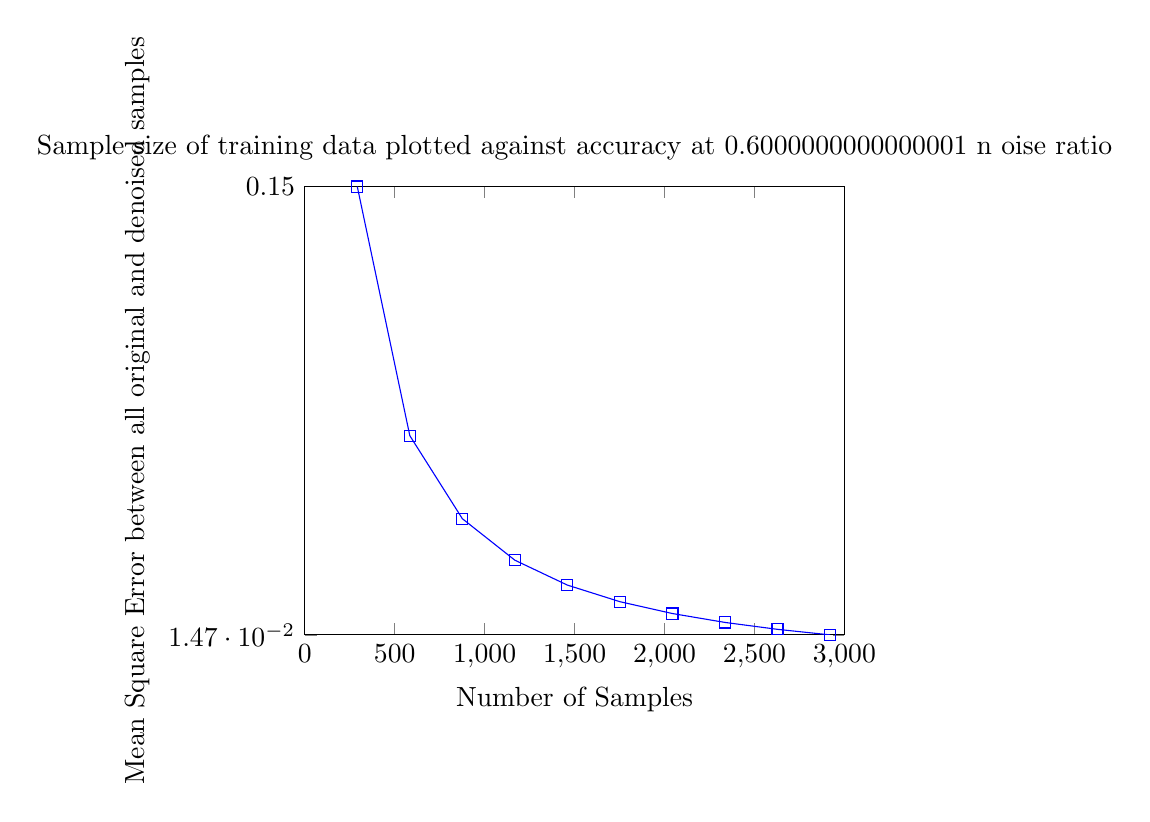
\begin{tikzpicture}
\begin{axis}[
title={Sample size of training data plotted against accuracy at 0.6000000000000001 n\
oise ratio},
xlabel={Number of Samples},
ylabel={Mean Square Error between all original and denoised samples},
xmin=0, xmax=3000,
ymin=0.014664246085810653, ymax=0.14740959835348086,
xtick={0,500,1000,1500,2000,2500,3000},
ytick={0.014664246085810653,0.14740959835348086},
legend pos=north west,
ymajorgrids=true,
grid style=dashed,
]

\addplot[
color=blue,
mark=square,
]
coordinates {

(292, 0.14740959835348086)
(584, 0.07365170886688645)
(876, 0.0490684032194625)
(1168, 0.03677862732142638)
(1460, 0.029406112558283688)
(1752, 0.024492137761461794)
(2044, 0.02098293704181635)
(2336, 0.01835168133512159)
(2628, 0.016305667194744276)
(2921, 0.014664246085810653)
    };
\end{axis}
\end{tikzpicture}


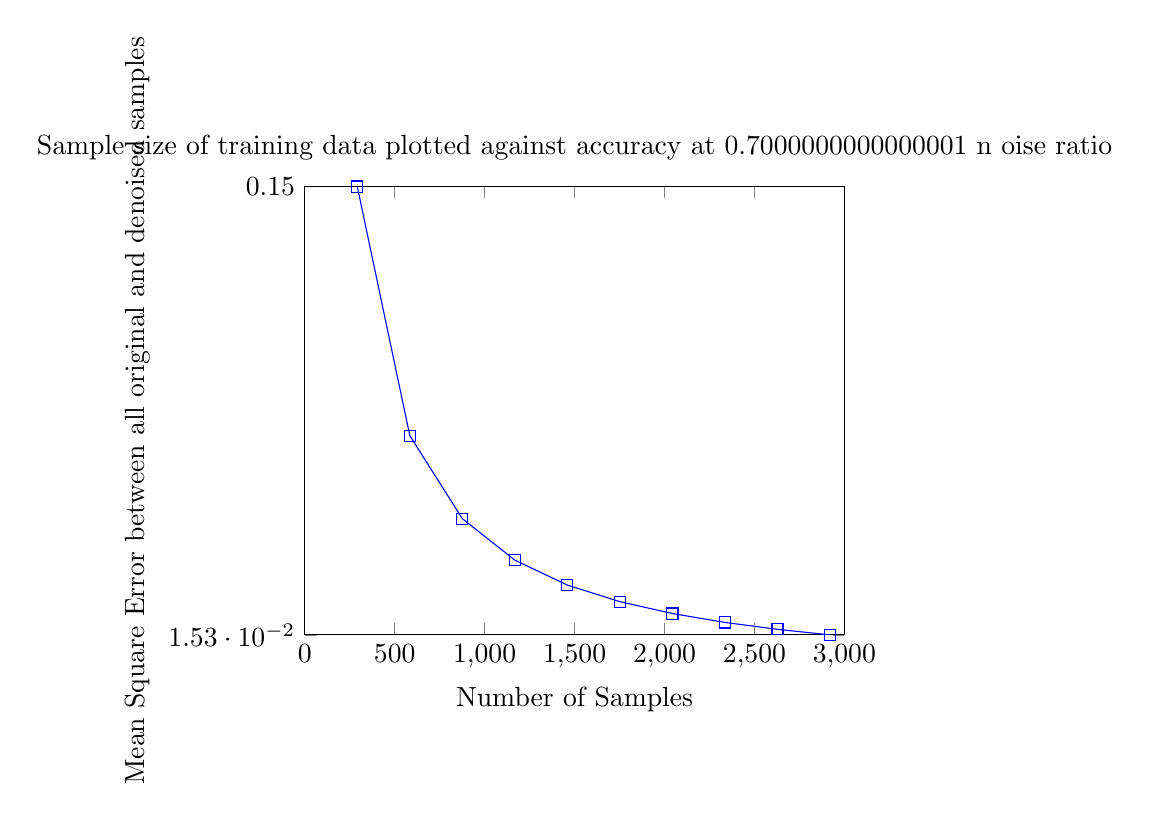
\begin{tikzpicture}
\begin{axis}[
title={Sample size of training data plotted against accuracy at 0.7000000000000001 n\
oise ratio},
xlabel={Number of Samples},
ylabel={Mean Square Error between all original and denoised samples},
xmin=0, xmax=3000,
ymin=0.015268924660288655, ymax=0.15316382367167933,
xtick={0,500,1000,1500,2000,2500,3000},
ytick={0.015268924660288655,0.15316382367167933},
legend pos=north west,
ymajorgrids=true,
grid style=dashed,
]

\addplot[
color=blue,
mark=square,
]
coordinates {

(292, 0.15316382367167933)
(584, 0.07655169558222895)
(876, 0.05101565404916926)
(1168, 0.03824860125957213)
(1460, 0.030589049137066848)
(1752, 0.02548320549841885)
(2044, 0.02183659188698234)
(2336, 0.019101944270679457)
(2628, 0.016975266628540795)
(2921, 0.015268924660288655)
    };
\end{axis}
\end{tikzpicture}




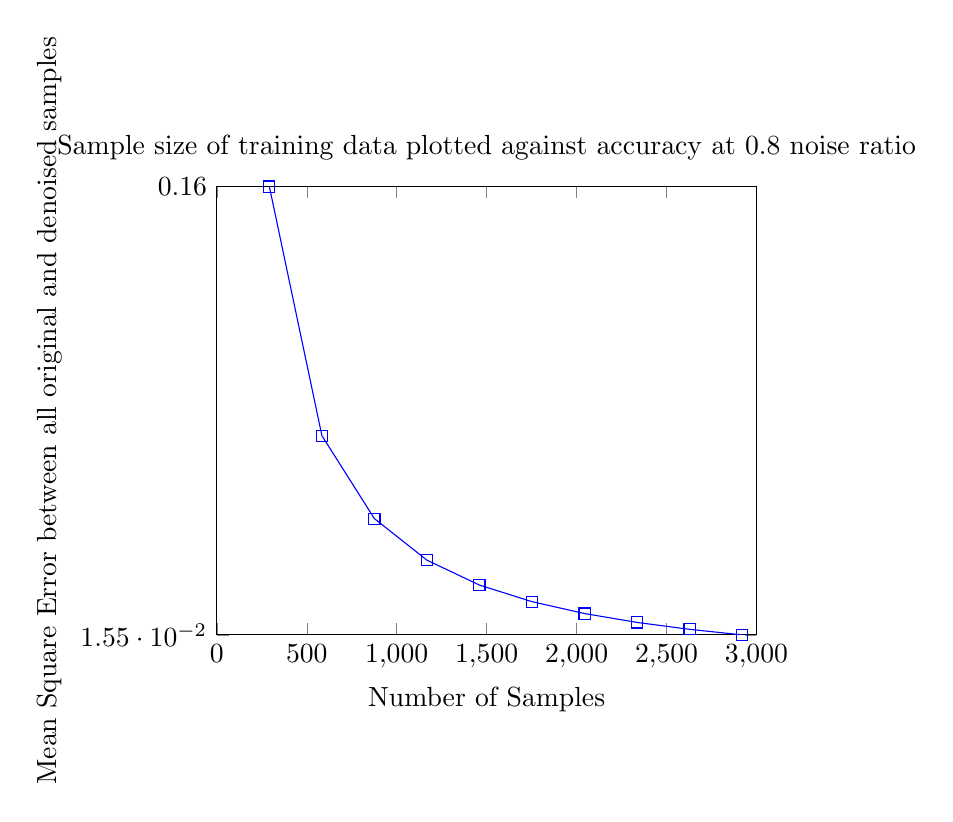
\begin{tikzpicture}
\begin{axis}[
title={Sample size of training data plotted against accuracy at 0.8 noise ratio},
xlabel={Number of Samples},
ylabel={Mean Square Error between all original and denoised samples},
xmin=0, xmax=3000,
ymin=0.015479411767285546, ymax=0.15510335725697144,
xtick={0,500,1000,1500,2000,2500,3000},
ytick={0.015479411767285546,0.15510335725697144},
legend pos=north west,
ymajorgrids=true,
grid style=dashed,
]

\addplot[
color=blue,
mark=square,
]
coordinates {

(292, 0.15510335725697144)
(584, 0.07753403334686536)
(876, 0.05167828016351627)
(1168, 0.03875087329222023)
(1460, 0.03099476894738528)
(1752, 0.02582429309587648)
(2044, 0.022131308052886253)
(2336, 0.01936174181855354)
(2628, 0.0172077734229597)
(2921, 0.015479411767285546)
    };
\end{axis}
\end{tikzpicture}



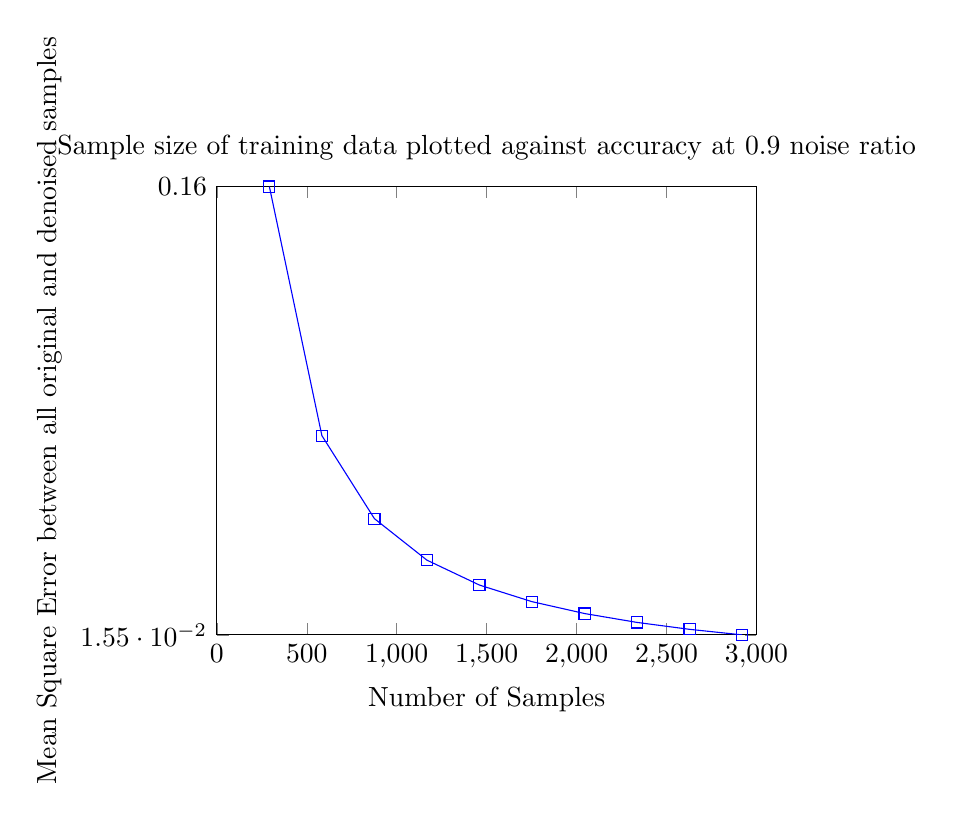
\begin{tikzpicture}
\begin{axis}[
title={Sample size of training data plotted against accuracy at 0.9 noise ratio},
xlabel={Number of Samples},
ylabel={Mean Square Error between all original and denoised samples},
xmin=0, xmax=3000,
ymin=0.015518944044437584, ymax=0.15540617158295383,
xtick={0,500,1000,1500,2000,2500,3000},
ytick={0.015518944044437584,0.15540617158295383},
legend pos=north west,
ymajorgrids=true,
grid style=dashed,
]

\addplot[
color=blue,
mark=square,
]
coordinates {

(292, 0.15540617158295383)
(584, 0.07769222436475232)
(876, 0.05178791371094459)
(1168, 0.03883599882694618)
(1460, 0.03106503414614501)
(1752, 0.025884529840647756)
(2044, 0.022184282344690106)
(2336, 0.01940918541204274)
(2628, 0.017250857459429263)
(2921, 0.015518944044437584)
    };
\end{axis}
\end{tikzpicture}

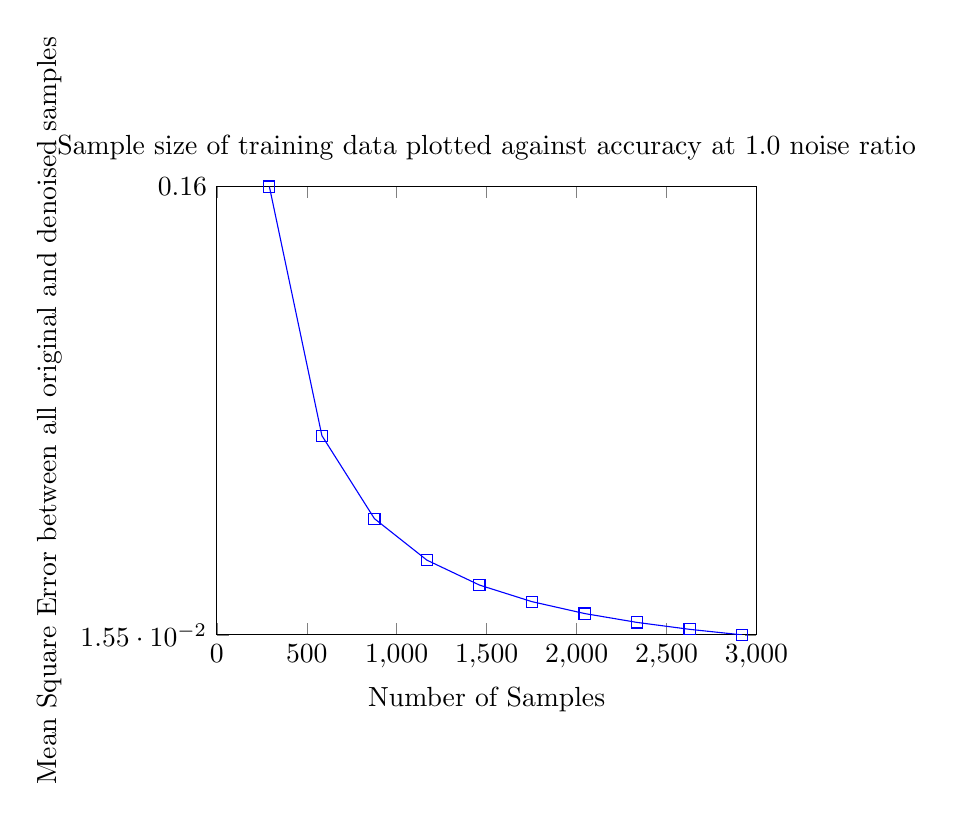
\begin{tikzpicture}
\begin{axis}[
title={Sample size of training data plotted against accuracy at 1.0 noise ratio},
xlabel={Number of Samples},
ylabel={Mean Square Error between all original and denoised samples},
xmin=0, xmax=3000,
ymin=0.015542170619278756, ymax=0.15558718483515635,
xtick={0,500,1000,1500,2000,2500,3000},
ytick={0.015542170619278756,0.15558718483515635},
legend pos=north west,
ymajorgrids=true,
grid style=dashed,
]

\addplot[
color=blue,
mark=square,
]
coordinates {

(292, 0.15558718483515635)
(584, 0.07778632477025116)
(876, 0.05185290467963103)
(1168, 0.03888633287842765)
(1460, 0.031106493034103642)
(1752, 0.0259200150587382)
(2044, 0.022215450343350485)
(2336, 0.01943708706691789)
(2628, 0.017276179675566546)
(2921, 0.015542170619278756)
    };
\end{axis}
\end{tikzpicture}





\end{document}